\makeatletter \graphicspath{ {\import@path} }
\makeatother

%%%%%%%%%%%%%%%%%%%%%%%%%%%%%%%%%%%%%%%%%%%%%%%%%%%%%%%%%%%%%%%%%%%%%%%%%%%%%%%
\begin{frame}[fragile]{Introduction}
  \begin{columns}
    \begin{column}{0.6\textwidth}
       \begin{itemize}
        \item Search Sensitivity for Supersymmetry with Compressed Mass Spectrum in the Vector Boson Fusion Topology in 0-lepton Final State with the CMS Experiment
        \item This analysis is a part of the CMS analysis that utilizes 0-, 1-, and 2-lepton final states.
      \end{itemize}	
         
    \end{column}
    \begin{column}{0.4\textwidth}
      \begin{figure}[htpb]
        \centering
        \includegraphics[width=0.8\textwidth]{fig/misc/AN-20-096-cover.pdf}
      \end{figure}
      
    \end{column}
  \end{columns}
\end{frame}

%%%%%%%%%%%%%%%%%%%%%%%%%%%%%%%%%%%%%%%%%%%%%%%%%%%%%%%%%%%%%%%%%%%%%%%%%%%%%%%
\begin{frame}[fragile]{The Standard Model of Particle Physics}
  \begin{figure}[htpb]
    \centering
    \includegraphics[width=0.8\textwidth]{fig/standard-model.pdf}
  \end{figure}
\end{frame}

%%%%%%%%%%%%%%%%%%%%%%%%%%%%%%%%%%%%%%%%%%%%%%%%%%%%%%%%%%%%%%%%%%%%%%%%%%%%%%%
\begin{frame}[fragile]{The Standard Model under Attack}
  The Standard Model 
  \begin{itemize}
    \item Hierarchy problem
    \item Oscillating Neutrino
    \item Dark Matter
    \item \(3.1 \sigma\) discrepancy for \PQb anomaly
    \item \(4.2\sigma\) discrepancy for muon anomalous magnetic momentum
  \end{itemize}
\end{frame}

%%%%%%%%%%%%%%%%%%%%%%%%%%%%%%%%%%%%%%%%%%%%%%%%%%%%%%%%%%%%%%%%%%%%%%%%%%%%%%%
\begin{frame}[fragile]{Supersymmetry}
  \begin{itemize}
    \item {\bf Supersymmetry (SUSY)} can solve many problem the SM has by restoring symmetry between fermions and bosons.
    \item The Minimal Supersymmetric Standard Model (MSSM) introduces two Higgs doublets to the SM and the supersymmetric partners.
    \item[\(\rightarrow\)] SUSY can solve the gauge hierarchy problem without a fine-tuning.
    \item[\(\rightarrow\)] When the R-parity is conserved, the lightest neutralino become stable and then is a canonical dark matter candidate.
  \end{itemize}

  \begin{figure}[htpb]
    \centering
    \includegraphics[height=0.4\textheight]{fig/susy_particles.png}
  \end{figure}

\end{frame}


%%%%%%%%%%%%%%%%%%%%%%%%%%%%%%%%%%%%%%%%%%%%%%%%%%%%%%%%%%%%%%%%%%%%%%%%%%%%%%%
\begin{frame}[fragile]{Supersymmetry}
  \begin{itemize}
    \item No direct experimental evidence of SUSY yet.
    \item The phase space relevant to coloured SUSY particles are constrained up to about 1 TeV.
  \end{itemize}
  
  \begin{figure}[htpb]
    \centering
    \includegraphics[width=0.4\textwidth]{fig/T2tt_limits_summary_cms.pdf}
    \includegraphics[width=0.4\textwidth]{fig/WZ_limits_summary_cms.pdf}
  \end{figure}
\end{frame}

%%%%%%%%%%%%%%%%%%%%%%%%%%%%%%%%%%%%%%%%%%%%%%%%%%%%%%%%%%%%%%%%%%%%%%%%%%%%%%%
\begin{frame}[fragile]{Motivation for the Compressed Mass Spectrum}
   Where is SUSY hiding?
\end{frame}


%%%%%%%%%%%%%%%%%%%%%%%%%%%%%%%%%%%%%%%%%%%%%%%%%%%%%%%%%%%%%%%%%%%%%%%%%%%%%%%
\begin{frame}[fragile]{Motivation for the Compressed Mass Spectrum}
   Where is SUSY hiding?
  \begin{itemize}
    \item[\(\blacksquare\)] SUSY does not exists.
  \end{itemize}
\end{frame}

%%%%%%%%%%%%%%%%%%%%%%%%%%%%%%%%%%%%%%%%%%%%%%%%%%%%%%%%%%%%%%%%%%%%%%%%%%%%%%%
\begin{frame}[fragile]{Motivation for the Compressed Mass Spectrum}
  \(\blacksquare\) Where is SUSY hiding?
  \begin{itemize}
    \item[{\includegraphics[width=0.5cm]{fig/misc/no-graduate.png}}] \sout{SUSY does not exists.} 
    \item[\(\blacksquare\)] SUSY particles too heavy to be probed with the current LHC energies \(\Rightarrow\) more powerful collider?
  \end{itemize}
\end{frame}

%%%%%%%%%%%%%%%%%%%%%%%%%%%%%%%%%%%%%%%%%%%%%%%%%%%%%%%%%%%%%%%%%%%%%%%%%%%%%%%
\begin{frame}[fragile]{Motivation for the Compressed Mass Spectrum}
  Where is SUSY hiding?
  \begin{itemize}
    \item[{\includegraphics[width=0.5cm]{fig/misc/no-graduate.png}}] \sout{SUSY does not exists.} 
    \item[{\includegraphics[width=0.5cm]{fig/misc/no-graduate.png}}] \sout{SUSY particles are too heavy to be probed with the current LHC energies}
    \item[\(\blacksquare\)] {\bf SUSY particles are hidden in the phase space where the experimental sensitivity is low}
  \end{itemize}

  \(\Rightarrow\) {\bf Compressed Mass Spectrum}
  \begin{itemize}
    \item SUSY particles can be nearly degenerate in mass.
    \item SM particles from SUSY particle decays have low energy to be undetected.
    \item The LSP produced at the end of a decay chain traverse the detector without interactions.
    \item How can we find the compressed mass spectrum SUSY?
  \end{itemize}
\end{frame}

%%%%%%%%%%%%%%%%%%%%%%%%%%%%%%%%%%%%%%%%%%%%%%%%%%%%%%%%%%%%%%%%%%%%%%%%%%%%%%%
\begin{frame}[fragile]{Vector Boson Fusion Topology}
  \begin{columns}
    \begin{column}{0.6\textwidth}
      \begin{itemize}
        \item In proton-proton collider, each of incoming quarks can be slightly deflected while emitting a heavy vector boson.
        \item Theses bosons can fuse to produce a Higgs boson or electroweakinos.
        \item This vector boson fusion (VBF) topoloy is characterized by two energetic jets which are located in forward, opposite hemispheres of the detector. 
        \begin{itemize}
          \item[\(\rightarrow\)] \({\footnotesize m(j_{1}j_{2}) \approx \sqrt{2\pt(j_{1})\pt(j_{2})}\cosh{\abs{\eta(j_{1}) - \eta(j_{2})}} }\)
        \end{itemize}
        \item This VBF topoloy is proposed to probe \(H\to\tau\tau\).
      \end{itemize}
    \end{column}

    \begin{column}{0.4\textwidth}
      \begin{figure}[htpb]
        \centering
        \includegraphics[width=0.9\textwidth]{fig/VectorBosonFusion.png}
      \end{figure}
    \end{column}
  \end{columns}

\end{frame}

%%%%%%%%%%%%%%%%%%%%%%%%%%%%%%%%%%%%%%%%%%%%%%%%%%%%%%%%%%%%%%%%%%%%%%%%%%%%%%%
{%<--- Start local changes
\setbeamertemplate{navigation symbols}{}
\usebackgroundtemplate{
  \centering
  \includegraphics[height=\paperheight]{fig/cms/lhc-google-earth.png}
}
\begin{frame}[plain]
\end{frame}
}%<---- Finish local changes

%%%%%%%%%%%%%%%%%%%%%%%%%%%%%%%%%%%%%%%%%%%%%%%%%%%%%%%%%%%%%%%%%%%%%%%%%%%%%%%
{%<--- Start local changes
\setbeamertemplate{navigation symbols}{}
\usebackgroundtemplate{
  \centering
  \includegraphics[height=\paperheight]{fig/cms/lhc-0-high.jpg}
}
\begin{frame}[plain]
\end{frame}
}%<---- Finish local changes

%%%%%%%%%%%%%%%%%%%%%%%%%%%%%%%%%%%%%%%%%%%%%%%%%%%%%%%%%%%%%%%%%%%%%%%%%%%%%%%
\begin{frame}[fragile]{The LHC Collider}
  \begin{figure}[htpb]
    \centering
    \includegraphics[height=0.75\textheight]{fig/cms/Christiane-1260465__CERN-complex.pdf}
  \end{figure}
  \(\bullet\) The largest and highest-energy particle collider in the world \\
  \(\bullet\) Built in a circular tunnel with circumference of 27 km and 45--175 m 
\end{frame}

%%%%%%%%%%%%%%%%%%%%%%%%%%%%%%%%%%%%%%%%%%%%%%%%%%%%%%%%%%%%%%%%%%%%%%%%%%%%%%%
{%<--- Start local changes
\setbeamertemplate{navigation symbols}{}
\usebackgroundtemplate{
  \centering
  \includegraphics[height=\paperheight]{fig/cms/lhc-google-earth.png}
}
\begin{frame}[plain]
\end{frame}
}%<---- Finish local changes

%%%%%%%%%%%%%%%%%%%%%%%%%%%%%%%%%%%%%%%%%%%%%%%%%%%%%%%%%%%%%%%%%%%%%%%%%%%%%%%
{%<--- Start local changes
\setbeamertemplate{navigation symbols}{}
\usebackgroundtemplate{
  \centering
  \includegraphics[width=\paperwidth]{fig/cms/cms-google-earth.png}
}
\begin{frame}[plain]
\end{frame}
}%<---- Finish local changes


%%%%%%%%%%%%%%%%%%%%%%%%%%%%%%%%%%%%%%%%%%%%%%%%%%%%%%%%%%%%%%%%%%%%%%%%%%%%%%%
{%<--- Start local changes
\setbeamertemplate{navigation symbols}{}
\usebackgroundtemplate{
  \includegraphics[height=\paperheight]{fig/cms/cms.jpeg}
}
\begin{frame}[plain]
\end{frame}
}%<---- Finish local changes


%%%%%%%%%%%%%%%%%%%%%%%%%%%%%%%%%%%%%%%%%%%%%%%%%%%%%%%%%%%%%%%%%%%%%%%%%%%%%%%
\begin{frame}[fragile]{The CMS detector}
  \begin{figure}[htpb]
    \centering
    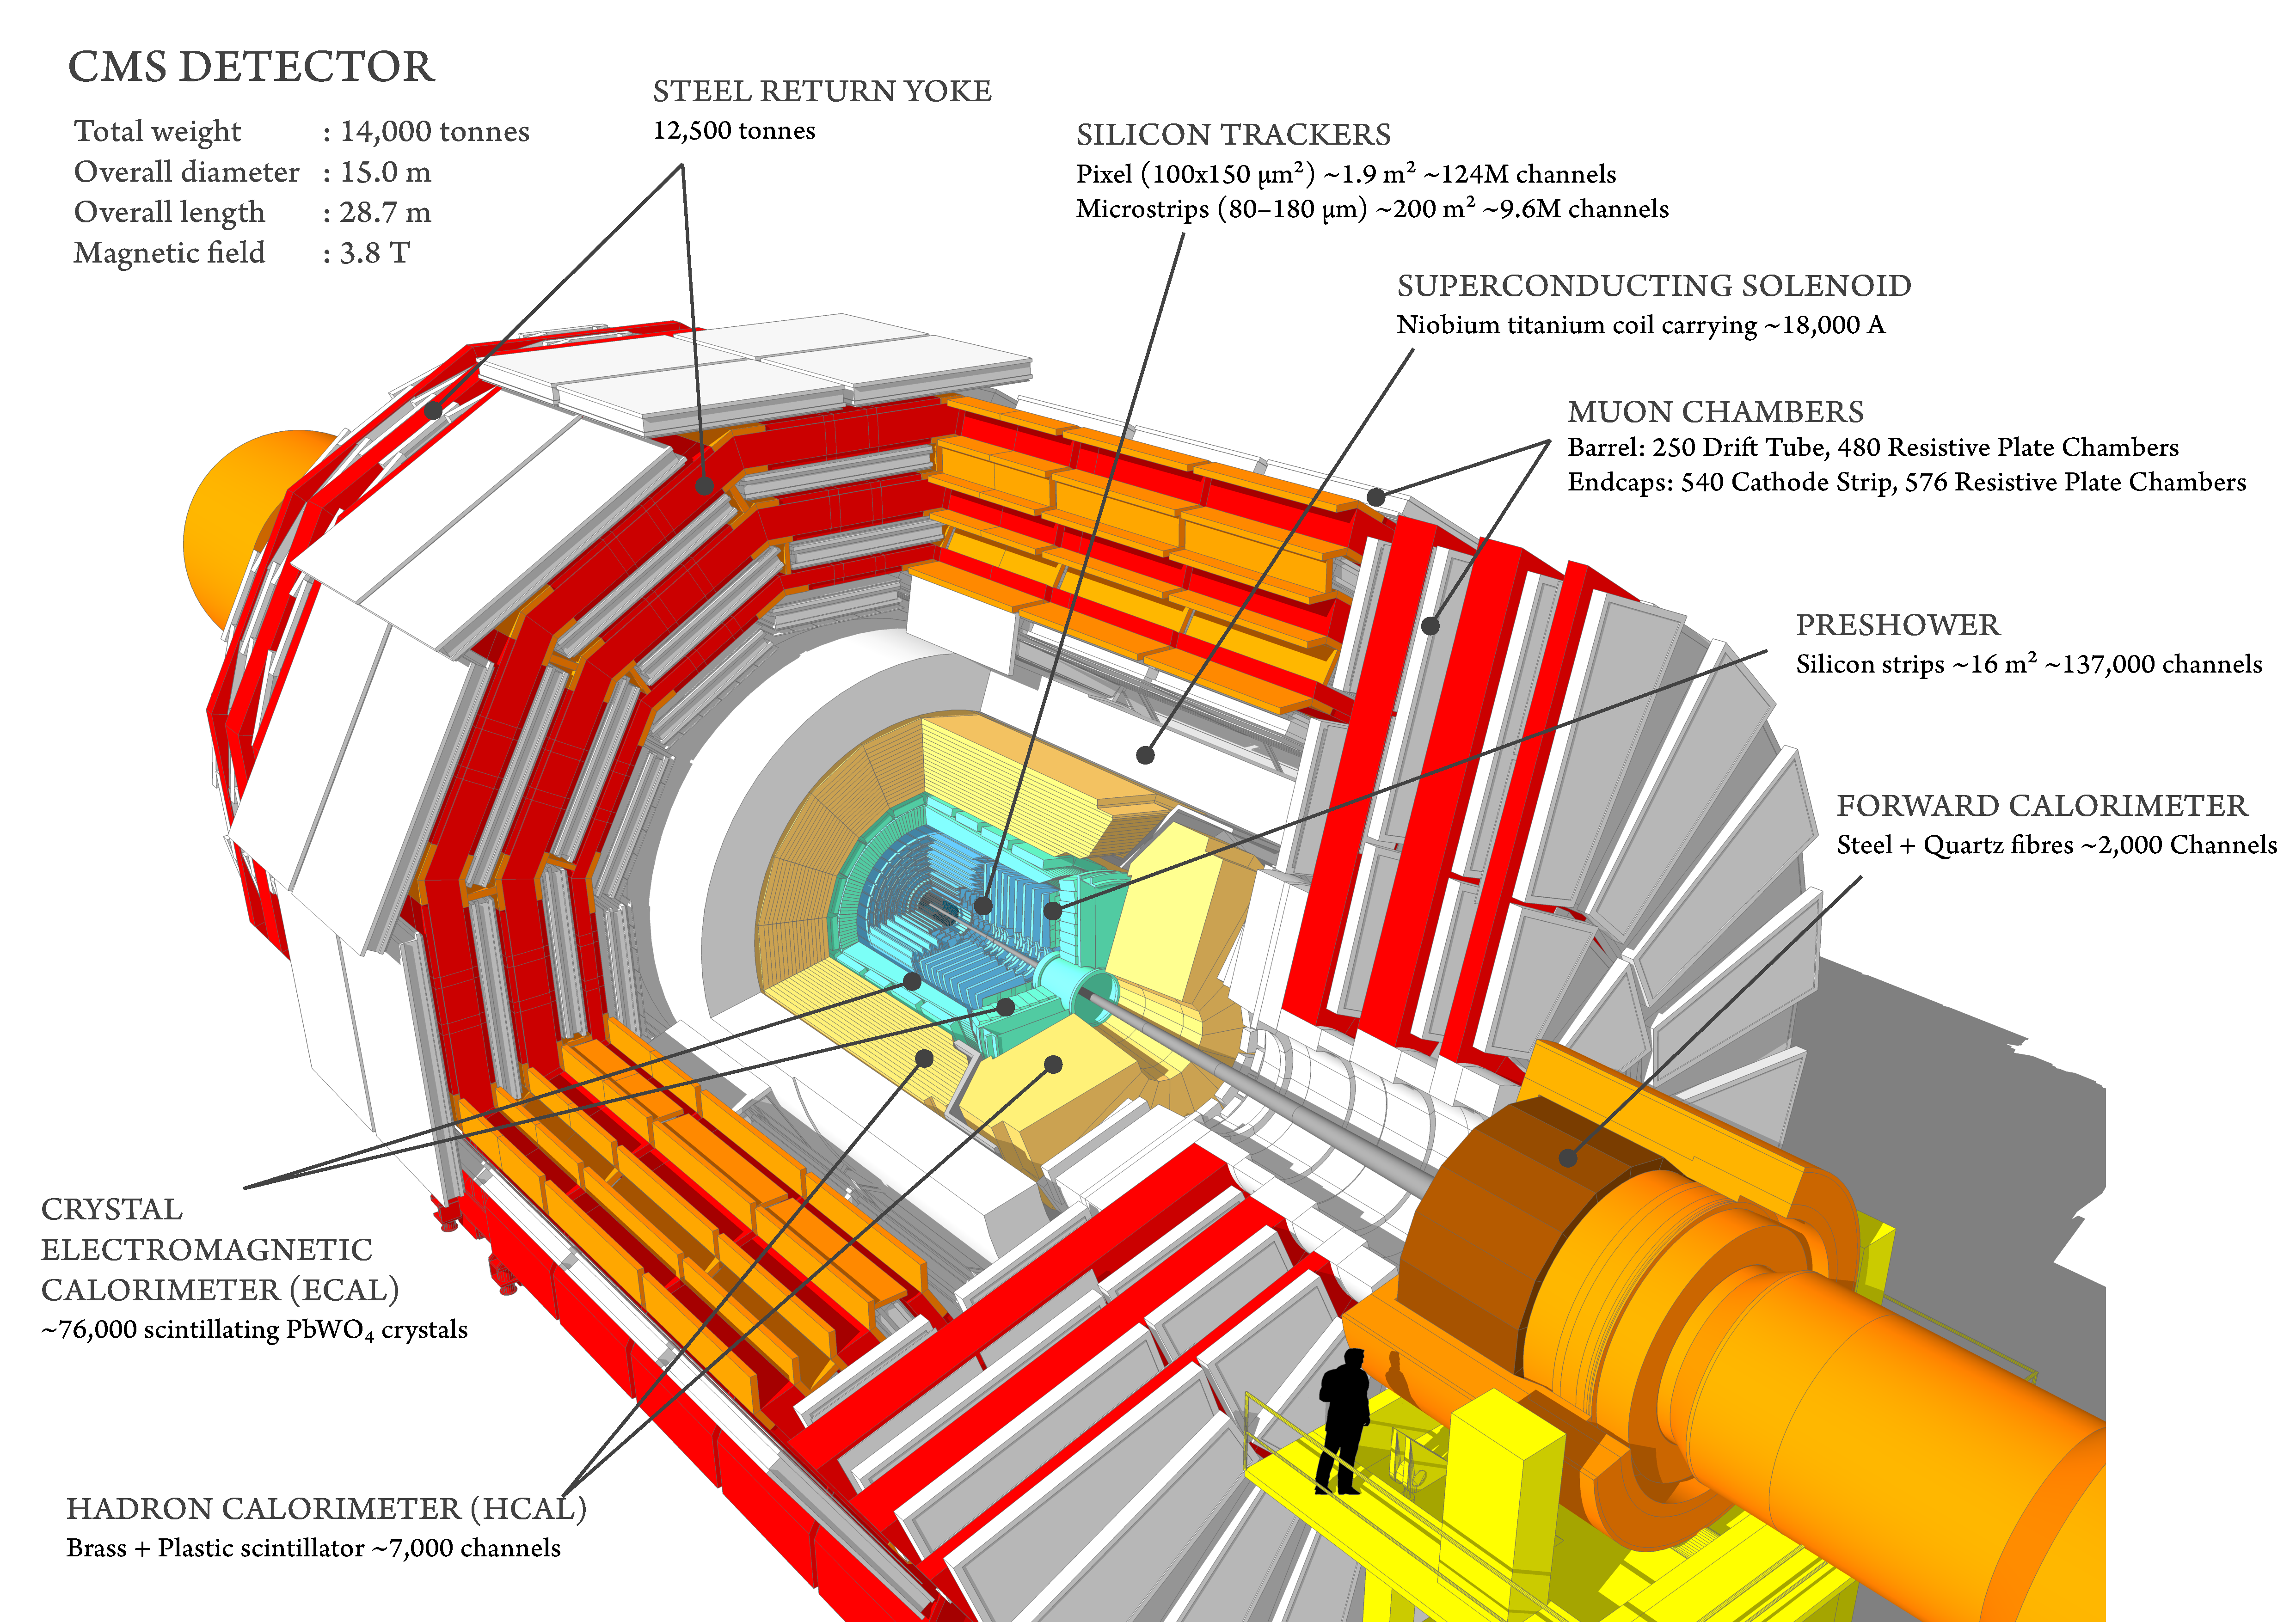
\includegraphics[width=0.9\textwidth]{fig/cms/cms_160312_06.pdf}
  \end{figure}
\end{frame}

%%%%%%%%%%%%%%%%%%%%%%%%%%%%%%%%%%%%%%%%%%%%%%%%%%%%%%%%%%%%%%%%%%%%%%%%%%%%%%%
\begin{frame}[fragile]{Reconstruction}
  \begin{figure}[htpb]
    \centering
    \includegraphics[height=0.8\textheight]{fig/cms/CMS-PRF-14-001_Figure_001.pdf}
  \end{figure}
\end{frame}

%%%%%%%%%%%%%%%%%%%%%%%%%%%%%%%%%%%%%%%%%%%%%%%%%%%%%%%%%%%%%%%%%%%%%%%%%%%%%%%
\begin{frame}[fragile]{Jet and Missing Transverse Momentum}
  \begin{columns}
    \begin{column}{0.5\textwidth}
      \begin{exampleblock}{Jet}
        \begin{itemize}
          \item A Jet is a spray of particles produced due to the hadronisation of a coloured particle.
          \item The jet is then reconstructed by clustering particles.
        \end{itemize} 
      \end{exampleblock}

      \begin{figure}[htpb]
        \centering
        \includegraphics[width=1.0\textwidth]{fig/Sketch_PartonParticleCaloJet.png}
      \end{figure}
    \end{column}

    \vrule{}

    \begin{column}{0.5\textwidth}
      \begin{exampleblock}{Missing Transverse Momentum}
         \begin{gather*}
          \ptvecmiss = -\sum_{i \in \textrm{particles}} \ptvec(i) \\
          \ptmiss = \abs{\ptvecmiss}
        \end{gather*}       
      \end{exampleblock}
    \end{column}
  \end{columns}
\end{frame}

%%%%%%%%%%%%%%%%%%%%%%%%%%%%%%%%%%%%%%%%%%%%%%%%%%%%%%%%%%%%%%%%%%%%%%%%%%%%%%%
\begin{frame}[fragile]{Analysis Workflow}
  \begin{figure}[htpb]
    \centering
    \includegraphics[width=0.8\textwidth]{fig/analysis-workflow.pdf}
  \end{figure}
\end{frame}

%%%%%%%%%%%%%%%%%%%%%%%%%%%%%%%%%%%%%%%%%%%%%%%%%%%%%%%%%%%%%%%%%%%%%%%%%%%%%%%
\begin{frame}[fragile]{Three SUSY Scenarios}
  \begin{itemize}
    \item Minimal supersymmetric SM with R-parity conservation
    \item Electroweakino pair production via the pure electroweak vector boson fusion
      \begin{itemize}
        \item \(\PSGczDo\PSGczDo jj\), \(\PSGczDo\PSGcpmDo jj\), \(\PSGczDo\PSGczDt jj\) \(\PSGcpmDo\PSGcpmDo jj\), \(\PSGcpmDo\PSGczDo jj\) and \(\PSGczDt\PSGczDt jj\)
      \end{itemize}
    \item \PSGczDo is the stable lightest SUSY particle (LSP).
    \item \PSGczDt and \PSGcpmDo are degenerate in mass.
    \item \(\Delta m (\PSGczDt, \PSGczDo) = m(\PSGczDt) - m(\PSGczDo) \)
    \item The SUSY parameter space is summarised as \(m(\PSGczDt) - \Delta  m (\PSGczDt, \PSGczDo)\) space.
  \end{itemize}

  Three simplified MSSM scenarios are defined depending on the lepton mass assumption.
  \begin{itemize}
    \item Virtual W/Z decay
    \item Democratic \PSl decay
    \item {\PSGt}-dominant decay
  \end{itemize}
\end{frame}

%%%%%%%%%%%%%%%%%%%%%%%%%%%%%%%%%%%%%%%%%%%%%%%%%%%%%%%%%%%%%%%%%%%%%%%%%%%%%%%
\begin{frame}[fragile]{SUSY Scenarios: Virtual W/Z}
  \begin{columns}
    \begin{column}{0.6\textwidth}
       \begin{itemize}
        \item \( m(\PSl) \gg m(\PSGczDt) \)
        \item \(\branchingratio(\PSGcpmDo\to\PSGczDo\PWpmst)=1\)
        \item \(\branchingratio(\PSGczDt\to\PSGczDo\PZst)=1\)
      \end{itemize}
     
    \end{column}

    \begin{column}{0.4\textwidth}
      \begin{figure}[htpb]
        \centering
        \includegraphics[width=1.0\textwidth]{fig/scenarios/FeynmanVirtualWZ.pdf}
      \end{figure}
      
    \end{column}
  \end{columns}
\end{frame}

%%%%%%%%%%%%%%%%%%%%%%%%%%%%%%%%%%%%%%%%%%%%%%%%%%%%%%%%%%%%%%%%%%%%%%%%%%%%%%%
\begin{frame}[fragile]{SUSY Scenarios: Democratic \PSl decay}

  \begin{columns}
    \begin{column}{0.6\textwidth}
      \begin{itemize}
        \item \(m(\PSl) = ( m(\PSGczDt) + m(\PSGczDo) ) / 2 \)
        \item \(\branchingratio(\PSGcpmDo\to\PSl\PGnl) = 1/3 \)
        \item \(\branchingratio( \PSGczDt \to \PSlpm \Plmp ) = 1/3 \)
        \item \(\branchingratio(\PSl \to \PSGczDo \Pl) = 1\)
      \end{itemize}
    \end{column}

    \begin{column}{0.4\textwidth}
      \begin{figure}[htpb]
        \centering
        \includegraphics[width=1.0\textwidth]{fig/scenarios/FeynmanDemocraticSlepton.pdf}
      \end{figure}
    \end{column}
  \end{columns}
\end{frame}

%%%%%%%%%%%%%%%%%%%%%%%%%%%%%%%%%%%%%%%%%%%%%%%%%%%%%%%%%%%%%%%%%%%%%%%%%%%%%%%
\begin{frame}[fragile]{SUSY Scenarios: \PSGt-dominant decay}
  \begin{columns}
    \begin{column}{0.6\textwidth}
      \begin{itemize}
        \item \(m(\PSGt) = \frac{ m(\PSGczDt) + m(\PSGczDo) }{ 2 }\)
        \item \(m(\PSe), m(\PSGm) \gg m(\PSGczDt)\)
        \item \( \branchingratio( \PSGczDt \to \PSGtpm \PGnGt ) = 1 \)
        \item \( \branchingratio( \PSGcpmDo \to \PSGtpm \PSGtmp ) = 1 \)
        \item \( \branchingratio( \PSGt \to \PSGczDo \PGt ) = 1\)
        \item Additionally, the direct \PSGt pair production is considered. \(\sigma(\text{direct}\, \PSGt\PSGt) \approx 2\sim20(\tilde{\chi}_{i}\tilde{\chi}_{j})\)
      \end{itemize}
      
    \end{column}
    \begin{column}{0.4\textwidth}
      \begin{figure}[htpb]
        \centering
        \includegraphics[height=0.4\textheight]{fig/scenarios/FeynmanStauDominated.pdf}
        \includegraphics[height=0.4\textheight]{fig/scenarios/FeynmanDirectStau.pdf}
      \end{figure}
      
    \end{column}
  \end{columns}

\end{frame}

%%%%%%%%%%%%%%%%%%%%%%%%%%%%%%%%%%%%%%%%%%%%%%%%%%%%%%%%%%%%%%%%%%%%%%%%%%%%%%%
\begin{frame}[fragile]{Event Selection}
  \begin{columns}
    \begin{column}{0.4\textwidth} 
      \begin{itemize}
          \item {\color{BurntOrange} Lepton veto}
          \item {\color{Periwinkle} $\ptmiss > 250\,\GeV$  }
          \item {\color{Rhodamine} Dijet}
            \begin{itemize}
              \item \(m(jj) > 500\,\GeV\)
              \item \(\abs{\Delta\eta(jj)} > 3.8\)
            \end{itemize}
      \end{itemize}

    \end{column}
    \begin{column}{0.6\textwidth}
      \begin{figure}[htpb]
        \centering
        \includegraphics[width=1\textwidth]{fig/final-state-topology.png}
      \end{figure}
 
    \end{column}
  \end{columns}
\end{frame}

%%%%%%%%%%%%%%%%%%%%%%%%%%%%%%%%%%%%%%%%%%%%%%%%%%%%%%%%%%%%%%%%%%%%%%%%%%%%%%%
\begin{frame}[fragile]{Results}
  \begin{itemize}
    \item Two most dominant backgrounds are \(\PZ(\to\nu\nu)+\text{jets}\) and \(\PW(\to\Pl\PGn)+\text{jets}\), where \Pl has low energy to be undetected.
    \item The virtual WZ decay scenario with \(m(\PSGczDt)=300\,\GeV)\) and \(\Delta m=5\,\GeV\) is shown as a benchmark.
    \item The experimental and theoretical uncertainties are conservatively considered.
  \end{itemize}

  \begin{figure}[htpb]
    \centering
    \includegraphics[width=0.32\textwidth]{fig/sr/SR-mjj-2016.pdf}
    \includegraphics[width=0.32\textwidth]{fig/sr/SR-mjj-2017.pdf}
    \includegraphics[width=0.32\textwidth]{fig/sr/SR-mjj-2018.pdf}
  \end{figure}
\end{frame}

%%%%%%%%%%%%%%%%%%%%%%%%%%%%%%%%%%%%%%%%%%%%%%%%%%%%%%%%%%%%%%%%%%%%%%%%%%%%%%%
\begin{frame}[fragile]{Expected Exclusion Limit Calculation (1)}
  \begin{itemize}
    \item For a given signal point, the median expected upper limit (UL) on the SUSY cross section is calculated using the likelihood fit with the largest dijet mass distribution.
  \end{itemize}

   \begin{figure}[htpb]
    \centering
    \includegraphics[width=0.4\textwidth]{fig/sr/SR-mjj-2016.pdf}
    \includegraphics[width=0.4\textwidth]{fig/limit-example/step-1.pdf}
  \end{figure}     
\end{frame}

%%%%%%%%%%%%%%%%%%%%%%%%%%%%%%%%%%%%%%%%%%%%%%%%%%%%%%%%%%%%%%%%%%%%%%%%%%%%%%%
\begin{frame}[fragile]{Expected Exclusion Limit Calculation (2)}
  The \(\pm\sigma\) expected UL is calculated.
  \begin{figure}[htpb]
    \centering
    \includegraphics[height=0.6\textheight]{fig/limit-example/step-2.pdf}
  \end{figure}
\end{frame}

%%%%%%%%%%%%%%%%%%%%%%%%%%%%%%%%%%%%%%%%%%%%%%%%%%%%%%%%%%%%%%%%%%%%%%%%%%%%%%%
\begin{frame}[fragile]{Expected Exclusion Limit Calculation (3)}
  The \(\pm2\sigma\) expected UL is calculated.
  	\begin{figure}[htpb]
  	  \centering
  	  \includegraphics[height=0.6\textheight]{fig/limit-example/step-3.pdf}
  	\end{figure}
\end{frame}

%%%%%%%%%%%%%%%%%%%%%%%%%%%%%%%%%%%%%%%%%%%%%%%%%%%%%%%%%%%%%%%%%%%%%%%%%%%%%%%
\begin{frame}[fragile]{Expected Exclusion Limit  Calculation (4)}
  The \(m(\PSGczDt)\) region, in which the expected UL on the cross section is lower than the theoretical prediction, is excluded.
  	\begin{figure}[htpb]
  	  \centering
  	  \includegraphics[height=0.6\textheight]{fig/limit-example/step-4.pdf}
  	\end{figure}
\end{frame}

%%%%%%%%%%%%%%%%%%%%%%%%%%%%%%%%%%%%%%%%%%%%%%%%%%%%%%%%%%%%%%%%%%%%%%%%%%%%%%%
\begin{frame}[fragile]{Expected Exclusion Limit Calculation (5)}
  The \(m(\PSGczDt)\) region, in which the expected UL on the cross section is lower than the theoretical prediction, is excluded.
  	\begin{figure}[htpb]
  	  \centering
  	  \includegraphics[height=0.48\textheight]{fig/limit-example/step-4.pdf}
  	  \includegraphics[height=0.48\textheight]{fig/exclusion-3d/Limit3D_wz.pdf}
  	\end{figure}
\end{frame}

%%%%%%%%%%%%%%%%%%%%%%%%%%%%%%%%%%%%%%%%%%%%%%%%%%%%%%%%%%%%%%%%%%%%%%%%%%%%%%%
\begin{frame}[fragile]{Expected Exclusion Limit: Virtual WZ Decay Scenario}
  \begin{columns}
    \begin{column}{0.5\textwidth}

      \begin{figure}[htpb]
        \centering
        \includegraphics[width=1.0\textwidth]{fig/exclusion-3d/Limit3D_wz.pdf}
      \end{figure}

    \end{column}
    \begin{column}{0.5\textwidth}
      \begin{itemize}
        \item The exclusion limit to \(m(\PSGczDt)=m(\PSGcpmDo)\) is set to (228, 218, 104) GeV for \(\Delta m\)= (0.5, 5, 50) GeV
      \end{itemize}
      
    \end{column}
  \end{columns}


\end{frame}


%%%%%%%%%%%%%%%%%%%%%%%%%%%%%%%%%%%%%%%%%%%%%%%%%%%%%%%%%%%%%%%%%%%%%%%%%%%%%%%
\begin{frame}[fragile]{Expected Exclusion Limit: Democratic \PSl Decay Scenario}
  \begin{columns}
    \begin{column}{0.5\textwidth}

      \begin{figure}[htpb]
        \centering
        \includegraphics[width=1.0\textwidth]{fig/exclusion-3d/Limit3D_democratic.pdf}
      \end{figure}

    \end{column}
    \begin{column}{0.5\textwidth}
      \begin{itemize}
        \item The exclusion limit is set to (228, 202) GeV for \(\Delta m\)= (0.5, 5) GeV
      \end{itemize}
      
      
    \end{column}
  \end{columns}


\end{frame}

%%%%%%%%%%%%%%%%%%%%%%%%%%%%%%%%%%%%%%%%%%%%%%%%%%%%%%%%%%%%%%%%%%%%%%%%%%%%%%%
\begin{frame}[fragile]{Expected Exclusion Limit: \PSGt-dominated Decay Scenario}
  \begin{columns}
    \begin{column}{0.5\textwidth}
      \begin{figure}[htpb]
        \centering
        \includegraphics[width=1.0\textwidth]{fig/exclusion-3d/Limit3D_democratic.pdf}
      \end{figure}

    \end{column}
    \begin{column}{0.5\textwidth}
      \begin{itemize}
        \item The exclusion limit is set to (178, 103) GeV for \(\Delta m\)= (5, 50) GeV
      \end{itemize}
    \end{column}
  \end{columns}
\end{frame}

%%%%%%%%%%%%%%%%%%%%%%%%%%%%%%%%%%%%%%%%%%%%%%%%%%%%%%%%%%%%%%%%%%%%%%%%%%%%%%%
\begin{frame}[fragile]{Outlook}
  \begin{itemize}
    \item Search sensitivity study for SUSY with the compressed mass spectrum in the 0-lepton final state is performed as a part of the CMS analysis 
    \item In the virtual W/Z / democratic \PSl / \PSGt-dominated decay scenario, the stringent expected limit is set to the \(m(\PSGczDt)=m(\PSGcpmDo)\) below 228/228/178 GeV for \(\Delta m\)=0.5/0.5/5 GeV.
    \item The low sensitivity region with high \(m(\PSGczDt)\) or high \(\Delta m(\PSGczDt, \PSGczDo)\) will be covered by 1- and 2-lepton analyses.
  \end{itemize}
\end{frame}
